\chapter{SSH Server with Public-Private key Authentication}
\label{chp:ssh}

\section{Installation}

SSH allows you to connect to your server from a remote computer, just think if your server sits in the cupboard under the stairs and does not have a monitor or even a keyboard this would be handy.  To install the SSH-server on the server, run the following in the terminal;

\begin{lstlisting}
sudo apt-get install openssh-server
\end{lstlisting}

That's it, the server will work out of the box, just make sure that you take a look at the section on securing the ssh server (Section~\ref{sec:ssh_hardening})


\section{Display a banner on login}

To make your OpenSSH server display the contents of the $$/etc/issue.net$$ file as a pre-login banner, simply add or modify the line:

\begin{lstlisting}
Banner /etc/issue.net
\end{lstlisting}

In the file

$$/etc/ssh/sshd\_config$$

Rather than editing the banner file, which displays before logging into the ssh connection, you can change the MOTD (Message of the Day) which displays after logging in.

Now you can change the default message, or simply add a message to the end of the file.  To add another message, then simply run the command;

\begin{lstlisting}
sudo nano /etc/motd.tail
\end{lstlisting}

The file will be empty by default, and add anything you like, from a simple message to a full blown ASCII art masterpiece.  Once completed, exit nano and next time you log in the default MOTD will be shown with your addition at the end.

The default information is derived from some scripts that run in order and are located here;
$$ /etc/update-motd.d/$$

simply cd to the directory and then ls to show the scripts.

In order to disable one of the scripts from running, then simply change the permissions of the script so that it is no longer executable.  Run the command;

\begin{lstlisting}
sudo chmod -x [FILE NAME HERE]
\end{lstlisting}

You can add your own scripts by simply adding them to this directory and giving the prefixed number that will put it order.

If you decide to enable a script that you disabled earlier then simply run the command;

\begin{lstlisting}
sudo chmod +x [FILE NAME HERE]
\end{lstlisting}

\section{Accessing the SSH shell remotely}

\subsection*{Windows;}

Now on the main computer that you will access the server from install Putty.  See Section~\ref{sec:putty}.  Putty will let us remotely access the command line.

\subsection*{Ubuntu/Linux;}

This is slightly simpler, create a script and run it in terminal (Don't forget to enable execution).  An example of the script is below;

\begin{lstlisting}
 #!/bin/bash

slogin -i [Path to ssh key] user@a.server.com
\end{lstlisting}

\section{SSH public-private keys}
\label{sec:sshkeys}

SSH keys allow authentication between two hosts without the need of a password. SSH key authentication uses two keys a private key and a public key.  The SSH connection will need to be secured as anyone that can guess your password will be able to connect to your computer if the port is open to the internet.  One option would be not to forward your ports through your routers firewall, however sometimes you may be away from home and want to access the server.  Private/Public keys are the way forward.


To generate the keys, from a terminal prompt enter:

\begin{lstlisting}
ssh-keygen -t dsa
\end{lstlisting}

This will generate the keys using a DSA authentication identity of the user. During the process you will be prompted for a password. Simply hit Enter when prompted to create the key.

By default the public key is saved in the file
$$
 ~/.ssh/id\_dsa.pub
$$

and
$$
 ~/.ssh/id\_dsa
$$

is the private key. Now copy the $id\_dsa$ file to the client, then append $id\_dsa.pub$ to;

$$
~/.ssh/authorized\_keys
$$

by running the following command;

\begin{lstlisting}
cat id_dsa.pub >> .ssh/authorized_keys
\end{lstlisting}

However if the computer is a fresh installation, then you can simply change the name of the $id\_dsa.pub$ file to $authroized\_keys$.

Now open the config file, running the command;

\begin{lstlisting}
sudo nano /etc/ssh/sshd_config
\end{lstlisting}

Change the following settings;

\begin{lstlisting}
ChallengeResponseAuthentication no
PasswordAuthentication no
UsePAM no
\end{lstlisting}

Reload the ssh server,

\begin{lstlisting}
sudo service ssh restart
\end{lstlisting}

As long as the private key is copied to all the clients wishing to connect to the ssh server, you should now be able to SSH to the host without being prompted for a password.

\section{Further Hardening}
\label{sec:ssh_hardening}

This step is very vital if your server has access to the internet, after I installed ssh on my server and configured it as above, I had many attempted attacks on my server.  Nothing major, some attempted cracking of passwords with incorrect user names. But since I had the public-private keys enabled and passwords disabled there was no way they were getting in.  However I was not happy about my access logs filling up with failed connections.  since changing the ssh port from the standard $22$ to another port I have not had a single attempted connection apart from my own.  F.Y.I. the log containing the connection attempts can be found in $/var/log/auth.log$

After any changes to the config file, the ssh server must be restarted by running:

\begin{lstlisting}
sudo service ssh restart
\end{lstlisting}

\subsubsection{Port Number}

To change the port simply edit the file $$/etc/ssh/sshd\_config$$ By typing the following;

\begin{lstlisting}
sudo nano /etc/ssh/sshd_config
\end{lstlisting}

and changing the line $$Port\ 22$$ to another port number.

Multiple port numbers can be defined in this file by simply adding more lines similar to the one above, i.e.

\begin{verbatim}
Port 22
Port 222
Port 2222
Port 22222
\end{verbatim}

If connecting to the server with a linux box, and use a common port across multiple servers the port can be set on the connecting computer so that the $-p$ flag does not need to be used.  This can be set in the $/etc/ssh/ssh_config$ file. \textbf{Take special note of the file name}

\subsubsection{Protocol 2}

Make sure that the line in your config file reads;

\begin{verbatim}
Protocol 2
\end{verbatim}

This forces the server to only use ssh protocol 2 and not protocol 1 which is obsolete.

\subsubsection{Limit Users}

This is a good way of restricting the users that are allowed to ssh into the server, simply add the following line to your config file;

\begin{verbatim}
AllowUsers USER USER USER ...
\end{verbatim}

Or deny certain users;

\begin{verbatim}
DenyUsers root USER USER ...
\end{verbatim}

The same can be done for groups;

\begin{verbatim}
AllowGroups GROUP
DenyGroups GROUP
\end{verbatim}

The order that openssh processes these directives is as follows;

\directory{DenyUsers / AllowUsers / DenyGroups / AllowGroups}

\subsubsection{Idle Logout/Login}

This is very useful for closing unused ssh connections, simply add the following two lines to the end of your config file;\

\begin{verbatim}
ClientAliveInterval 180
ClientAliveCountMax 0
\end{verbatim}

This tells the server to log out any clients that have been inactive for the last half an hour.

\subsubsection{Disable .rhosts}

This is set as default, but worth a check;

\begin{verbatim}
IgnoreRhosts yes
\end{verbatim}

\subsubsection{Disable root login}

This is somewhat a polarising point, but better safe than sorry, don't let the root login through ssh;

\begin{verbatim}
PermitrootLogin no
\end{verbatim}

\subsubsection{Updates}

Just make sure that you constantly update your ssh server instance, use \textit{apt-get}.


\section{Running Scripts after Login}

There is a file that is executed upon login by a user over ssh, it can be found here;

$$/etc/ssh/sshrc$$

If the file exists, then it will be executed as a script upon login.

Alternatively, you can edit each individual users $~/.ssh/rc$, this file executes if it exists and the user logs in through ssh.

%---------------------------------------------------

\section{Using Putty (On Windows)}
\label{sec:putty}

Using Putty is easy, assuming that you downloaded and installed it to your Windows machine.  We will have two computers in action now, the 'remote' ubuntu server, and the 'local' windows machine.

Now lets create a new session, and save it for use later...

Type the host name or IP address of your remote ubuntu server, and then enter the port.  Now lets give the session a name (I like to use the name of the computer) so that we can refer to it later. For now lets click on save! See the screen-shot in figure~\ref{fig:putty1};

\begin{figure}[!th]
\centering
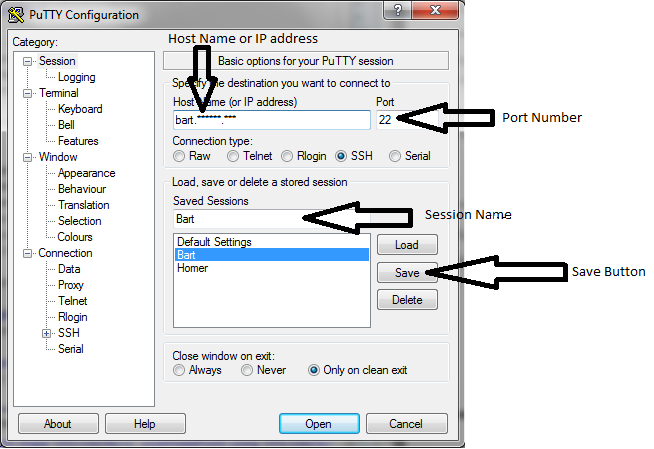
\includegraphics[scale=0.9]{./supportfiles/putty1}
\caption{Screen-shot of the first page of Putty's interface}
\label{fig:putty1}
\end{figure}

Now if you followed the method in Section~\ref{sec:sshkeys}, you need to sort out getting your key from your remote machine onto your local machine. (USB Stick, scp, ftp...)

We then tell putty to use this key when connecting to your remote server.  Go to the \textbf{Auth} page, \menu[,]{Connection, SSH, Auth}.  Then give putty the path to your key.  (Note you will have to open it in PuttyGen and convert it to the correct format, by saving it as a private key.)

Now go to \textbf{Data}, \menu[,]{Connection, Data}, and fill in the \textit{auto-login username}.

\section{Forwarding X11 to Windows}
\label{sec:X11forwarding}

If you need to run a GUI program over ssh then there is a way to do it;

On the remote machine, change a line in the sshd$\_$config file to read;

\begin{lstlisting}
X11Forwarding yes
\end{lstlisting}

Now on the local (windows) machine, you need to download and install \textit{Xming}. Once installed it doesn't need any more configuration.

Back to Putty, we need to set it up to handle X11 forwarding.  Go to \menu[,]{Connection, SSH, X11}, then check the Enable X11 option, and type into X display location \textit{localhost:0}.

Now simply connect to the server and run a GUI program such as xclock to test it is working.